\documentclass[addpoints,12pt]{exam}
\pagestyle{empty}
\usepackage{amsmath}
\usepackage{amssymb}
\usepackage{latexsym}
\usepackage[dvips]{graphicx}
\usepackage{enumerate}
\usepackage{amsfonts}
\newcommand{\nl} {\newline}
\newcommand{\normal}{\triangleleft}
\newcommand{\homo}{\simeq}
\newcommand{\R}{\mathbb{R}}
\newcommand{\Z}{\mathbb{Z}}
\newcommand{\Q}{\mathbb{Q}}
\newcommand{\N}{\mathbb{N}}
\newcommand{\C}{\mathbb{C}}
\newcommand{\ov}{\overline}
\newcommand{\E}{\varepsilon}
\newcommand{\F}{\varphi}
\newcommand{\MF}{\mathbb{F}}
\newcommand{\s}{\sqrt}

\newcommand{\vv}[2]{\begin{bmatrix} #1 \\ #2 \end{bmatrix}}
\newcommand{\vvv}[3]{\begin{bmatrix} #1 \\ #2 \\ #3\end{bmatrix}}
\newcommand{\vvvv}[4]{\begin{bmatrix} #1 \\ #2 \\ #3 \\ #4\end{bmatrix}}
\newcommand{\vvvvv}[5]{\begin{bmatrix} #1 \\ #2 \\ #3 \\ #4 \\ #5  \end{bmatrix}}

\everymath{\displaystyle}
\input{../../../AxesFunction}

\def\arraystretch{1.5}
\setlength\arraycolsep{20pt}
%\renewcommand{\baselinestretch}{1.3}

\begin{document}

~\hfill Student Name: \rule{2in}{.1pt}\\\\
\phantom{.}\hfill PERM: \rule{2in}{.1pt}\\\\
%\phantom{.}\hfill Section Time (e.g. 8am): \rule{2in}{.1pt}\\
Circle the section you ATTEND (if you are enrolled a different section, note which one):
\vskip.15in

\textbf{\begin{tabular}{cccccc}
Kyle: & Tue:8am & Tue:4pm & Tue:7pm\\
David: & Tue:5pm & Tue:6pm\\
Yihan: & Mon:4pm & Mon:5pm & Mon:6pm & Mon:7pm\\
Tom: & Tue:8am & Tue:4pm & Wed:8am\\
Matt: & Tue:5pm & Tue:6pm & Tue:7pm\\
\end{tabular}}
\vskip.25in



%Spring 2011
%Instructor: Stepan Paul
%Circle Your Section:\quad 8AM:Rahul\quad 4PM:Rahul\quad 5PM:Rahul\quad 6PM:Rahul\quad 6PM:Brandon
%\vskip0.5truein

\centerline{\bf \underline {Math 4B, Final, Spring 2017}}

\centerline{\bf \underline{Version A}}
\vskip0.2in

\underline {Instructions}: Read the instructions for each question carefully. No calculators, cell phones, or other electronic devices are permitted. No notes or textbooks. Academic dishonesty will not be tolerated. Show your work, write legibly, and circle your answers. 

\vspace{.5in}
\centerline{\gradetable}

\vspace{.5in}


\setlength\arraycolsep{2pt}
\def\arraystretch{1.2}

\textbf{I understand UCSB's policies regarding academic dishonesty, and I certify that this test was taken with academic integrity.}
\vspace{.5in}

Sign and date: \rule{5in}{.5pt}

%\medskip
%\medskip \vskip0.25truein
%\vskip0.25truein

%\vspace{0.5in} \large{\centerline{\begin{tabular}{|c|c|c|} \hline
%Problem  & Points & Score
%\\ \hline
% 1 & 25 &     \\ \hline
% 2 & 10 &      \\ \hline
% 3 & 15 &      \\ \hline
% 4 & 10 &      \\ \hline
% Total & 60 &  \\ \hline
%\end{tabular}}}
%}

\newpage
\begin{questions}
 
 \question[10] Find the solution to the initial value problem
 
 $$\begin{array}{ccccccc}
  x' & = & 3x & - & y&+&2 \\
  y' & = & x & + & y&+&2
 \end{array},\qquad x(0)=3,\;y(0)=0$$
 
 \newpage
 
  \question[18] Answer the following.
 \begin{parts}
  \part Find the solution to the initial value problem $x\frac{dy}{dx}+3y=6x$, $y(1)=2$
  \vfill
  
  \part Find the general solution to the ODE: $y''-6y'+8y=e^{2t}$.
  \vfill
  
  \newpage
  \part Find the general solution to the differential equation $y'=x^2e^y$. Solve for $y(x)$ explicitly.
  \vfill
  

 \end{parts}
 
 \newpage
 
 \question[12] Squirrels and rabbits both live on the Ellwood bluffs. If $S$ is the number of squirrels (in hundreds), and $R$ is the number of rabbits (in hundreds), their populations are modeled by the non-linear system
 \begin{align*}
  \frac{dR}{dt}&=14R-2R^2-RS\\
  \frac{dS}{dt}&=16S-2S^2-RS
 \end{align*}
 \begin{parts}
  \part Find the four equilibria of the system.
  \vfill
  \part One of these equilibria has $S>0$ and $R>0$. Use the Jacobian matrix to classify the behavior near this equilibrium point.
  \vfill
  \vfill
  \newpage
  \part Give a rough sketch of the phase plane for $S$ and $R$. Your picture should take into account your answer to parts (a) and (b), and should take into account the regions in which $S$ and $R$ are each increasing or decreasing. You do not need to consider cases in which $S$ or $R$ is negative.
  
  \simpleaxeslabels5500{$R$}{$S$}{}
  
  \vfill
  \part Write one or two sentences interpreting your findings in terms of how the populations of rabbits and squirrels interact.
  \vfill
 \end{parts}
 
 
 \newpage
 

 
 \question[5] Consider the linear homogeneous differential equation
$$x^2y''+2xy'-6y=0$$

\begin{parts}
\part Confirm that $y(x)=x^{-3}$ is a solution to the DE.
\vfill

\part Find another solution of the form $y(x)=x^k$.
\vfill

\part Find the solution which satisfies the initial conditions $y(1)=1$ and $y'(1)=12$.
\vfill

\end{parts}

 
 \newpage
 
 \question[6] The population $P$ of bees in a particular hive as a function of time $t$ satisfies the differential equation $\frac{dP}{dt}=P(P-100)(300-P)$, whose slope field is shown below.

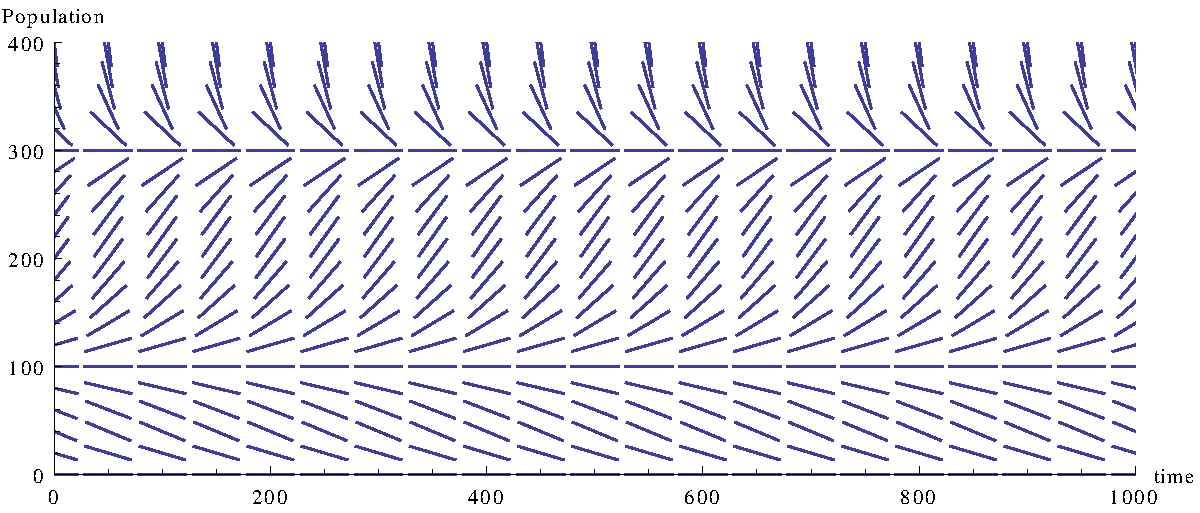
\includegraphics[scale=0.6]{SlopeField2}

\begin{parts}
\part What are equilibrium solutions to the differential equation? Explain your answer in two ways: one using the equation, and one using the graph.
\vfill


\part If there were $105$ bees initially, what is $\lim_{t\rightarrow\infty}P(t)$? Justify your answer by drawing a solution curve.
\vfill

\part If there were $95$ bees initially, what will the population be when $P(t)$ hits an inflection point?
\vfill

\end{parts}

 
 \newpage
 
 \question[2] Use differential equations to respond to the following:
 
  A torpedo is fired horizontally from a submarine. The torpedo has no propulsion of its own, and it is neutrally bouyant, so it does not float or sink, but it starts out moving forward due to it initial forward velocity. Because of hydrodynamic resistance, {its deceleration is proportional to the square of its speed}, slowing the torpedo down. Does the torpedo ever come to a complete stop? How far will it go? 

  
 

 
 
\end{questions}

\newpage

If you finish early, you must stay in your seat until the end. You should check your work, but if you are done, you can amuse yourself by coloring in these regular pentagonal tilings.

\begin{tabular}{cc}
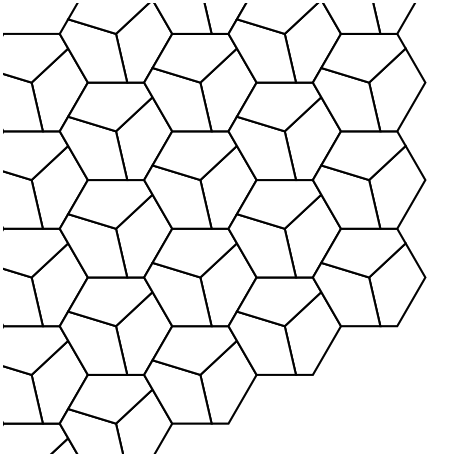
\includegraphics[width=.4\textwidth]{T1} & 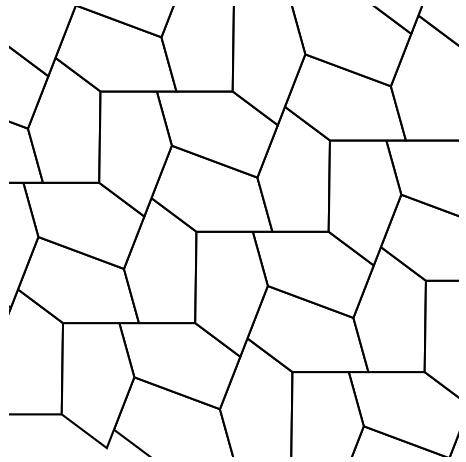
\includegraphics[width=.4\textwidth]{T2} \\
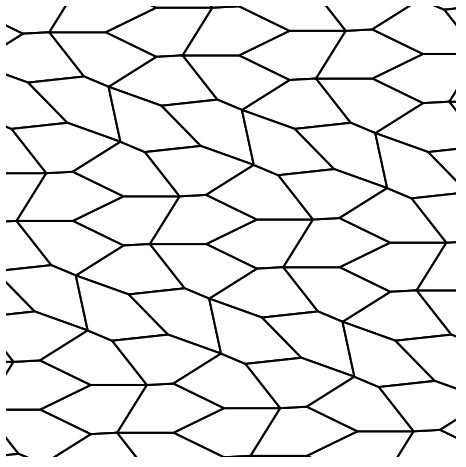
\includegraphics[width=.4\textwidth]{T3} &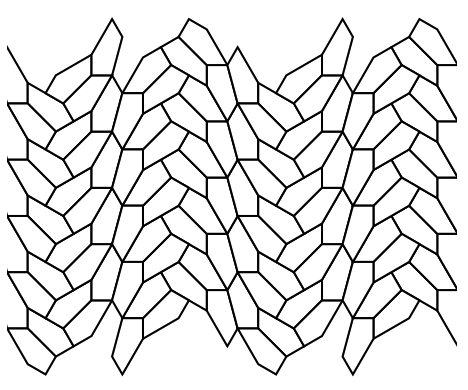
\includegraphics[width=.4\textwidth]{T15} 
\end{tabular}



\end{document}
